% Fig. 1 v6: instruction -> frozen VLA; one episode compared along identity / extent / permission; gallery of four more episodes.
% Source: paper/figures/fig01_teaser/v6/fig01_v6.pdf (+ fig01_v6.json: per-panel run, frame, crop, sha256). 6.875 x 3.01 in.
% Scripts: paper/tools/plotting/fig1_v4_assets.py (overlays), cvpr_v6_fig1_compose.py (layout, gallery frames).
\begin{minipage}{\textwidth}
\centering
\captionsetup{type=figure,hypcap=false}
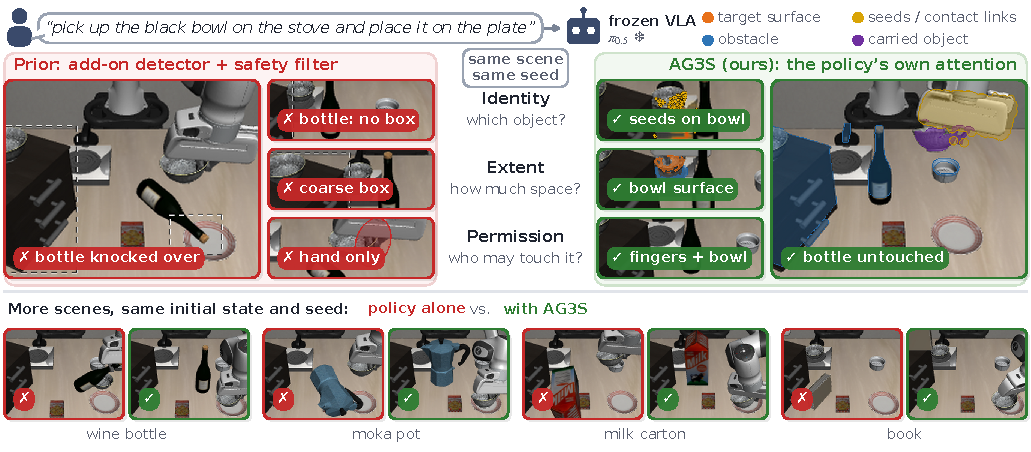
\includegraphics[width=\textwidth]{../figures/fig01_teaser/v6/fig01_v6.pdf}
\caption{\textbf{The policy that is told what to grasp already knows where it is.}
\emph{Top:} one SafeLIBERO episode, same initial state, seed, and moment. A detector-based safety layer (AEGIS~\cite{hu2026vlsa}; robot model of KNOWS$^\ast$~\cite{park2026knows}) misses the bottle, boxes the bowl with the cabinet, and models only the hand; the bottle falls.
\sys\ seeds the bowl from the frozen policy's own attention, bounds its observed surface, and lets only the contact links and the carried bowl touch it; the bottle stays upright.
\emph{Bottom:} selected episodes with other tasks and obstacles in which the policy alone collides and \sys\ succeeds without collision (examples, not a rate; see Sec.~\ref{sec:experiments}).}
\label{fig:teaser}
\end{minipage}
